\section{Modelo Completo}
\label{sec:non_arx}
%===============================================================================

Como apresentado na se��o (\ref{sec:arx}) o modelo ARX n�o consegue representar o
sistema (\ref{eq:system}) completamente, e a estimativa dos par�metros da Fun��o
de transfer�ncia s�o polarizados. Para contornar este problema utilizaremos um
modelo para descrever o sistema (\ref{eq:system}) de forma completa. \cite{system_identification}

O modelo escolhido para representar o sistema real � apresentado em (\ref{eq:compl}).

\begin{equation}
G(q, \theta )=\frac{a}{q-b}\;\;\;\;\;H(q, \theta)=\frac{q-c}{q-d}
\label{eq:compl}
\end{equation}

Utilizando o estimador �timo (\ref{eq:estimador}) obt�m-se a equa��o de diferen�as apresentada
em (\ref{eq:gmq_eq}). Utilizando o {\it{script}} \ref{anx_gmq_simul} obt�m-se o resultado
para os par�metros $a$, $b$, $c$ e $d$ para a fun��o $G(q, \theta)$ e $H(q, \theta)$.

\begin{equation}
\hat{y}(t/t-1, \theta)=H^{-1}(q, \theta)G(q, \theta)u(t)+[1-H^{-1}(q, \theta)]y(t)
\label{eq:estimador}
\end{equation}

\begin{equation}
\begin{matrix}
\hat{y}(t/t-1, \theta)= & a\;u(t-1)-ad\;u(t-2) +(d-c)y(t-1)\\
 & -b(d-c)y(t-2)+(b+c)\hat{y}(t-1/t-2, \theta)\\
 & -cb\;\hat{y}(t-2/t-3, \theta)
\end{matrix}
\label{eq:gmq_eq}
\end{equation}

Nas Figuras (\ref{fig:gmq_ab}) e (\ref{fig:gmq_cd}) apresentam-se os valores estimados para os par�metros
das fun��es de transfer�ncia $G(q)$ e $H(q)$ respectivamente.

\begin{figure}[htbp]
	\center
	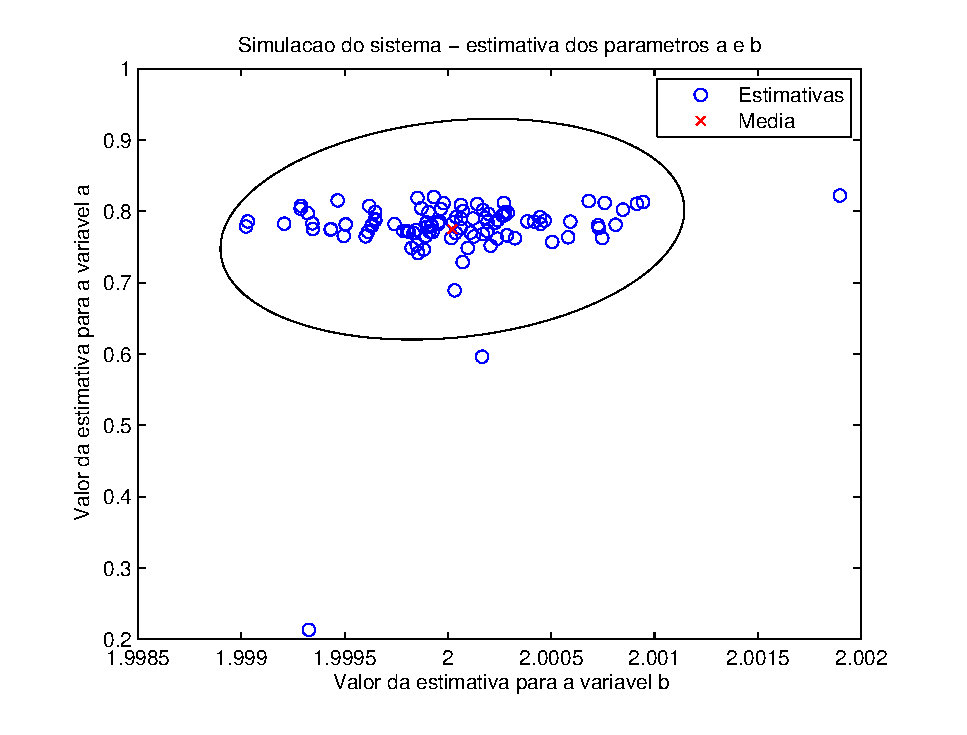
\includegraphics[width=0.98\columnwidth]{figures/gmq_ab.eps}
	\caption{Simula��o do sistema para uma entrada aleat�ria e utilizando o modelo completo - 
		vari�veis do processo $G(q)$ $a$ e $b$.}
	\label{fig:gmq_ab}
\end{figure}

\begin{figure}[htbp]
	\center
	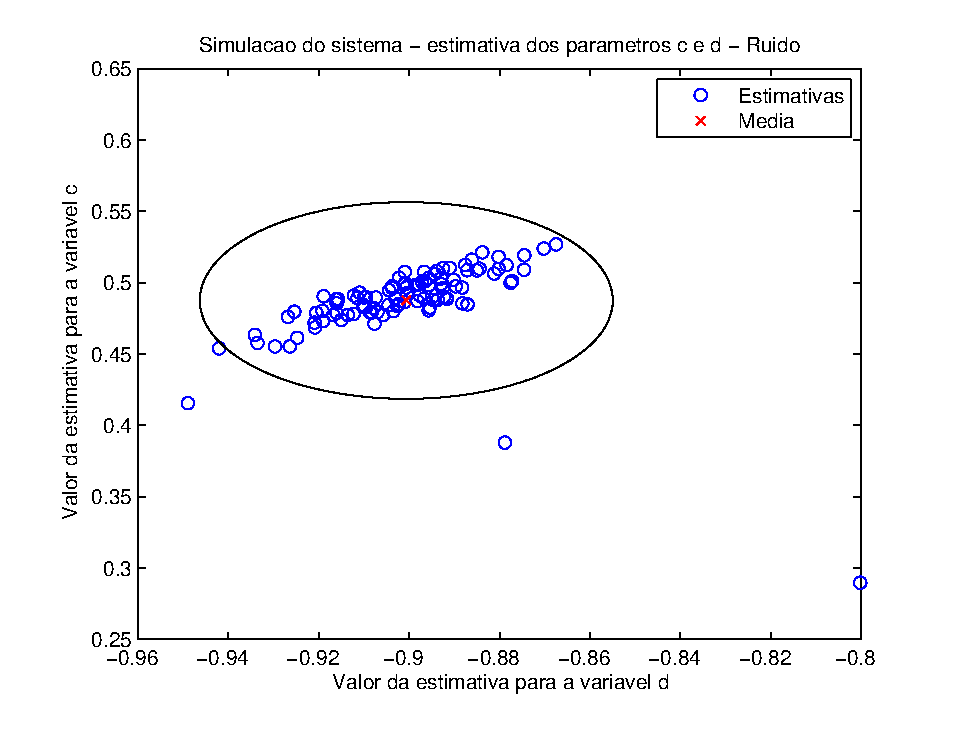
\includegraphics[width=0.98\columnwidth]{figures/gmq_cd.eps}
	\caption{Simula��o do sistema para uma entrada aleat�ria e utilizando o modelo completo - 
		vari�veis do ruido $H(q)$ $c$ e $d$.}
	\label{fig:gmq_cd}
\end{figure}

A m�dia das estimativas para os par�metros em quest�o � apresentado na Tabela (\ref{tab:gmq}).

\begin{table}[htbp]
  \begin{center}
	\caption{M�dia da estimativa para os par�metros de $G(q)$ e $H(q)$}
	\label{tab:gmq}
	\begin{small}
	  \begin{tabular}{cl}
		\hline
		Par�metro	& M�dia	\\
		\hline
		a			& 2.0000 \\
		b			& 0.7748 \\
		c			& -0.9006 \\
		d			& 0.4875 \\
		\hline
	  \end{tabular}
	\end{small}
  \end{center}
\end{table}


